% Created 2012-07-11 Wed 16:48
\documentclass[11pt]{article}
\usepackage[utf8]{inputenc}
\usepackage[T1]{fontenc}
\usepackage{graphicx}
\usepackage{longtable}
\usepackage{float}
\usepackage{wrapfig}
\usepackage{soul}
\usepackage{amssymb}
\usepackage{hyperref}
\usepackage{setspace}
\usepackage[spanish,activeacute]{babel}
\usepackage[left=1.5cm,top=2cm,right=1.5cm,bottom=1cm]{geometry}
\usepackage{fancyhdr}
\usepackage{amssymb}
\usepackage{anysize}
\usepackage{graphicx}
\usepackage{multicol}
\usepackage{float}
\usepackage{color}
\usepackage{listings}
\usepackage{appendix}
\usepackage{hyperref}
\hyphenpenalty=10000
\usepackage[nottoc,numbib]{tocbibind}

\title{}
\author{}
\date{}

\begin{document}





\begin{titlepage}
\begin{figure}[t]

\includegraphics[scale=0.35]{./img/FCFM.jpg}
%\begin{tabular}{l}
%Universidad de Chile \\
%Facultad de Ciencias Físicas y Matemáticas \\
%Departamento de Ciencias de la Computación \\

%\vspace{1.9cm}\mbox{}
%\end{tabular}
\end{figure}

\vspace*{0.2 in}

\begin{center}
\Large CC6908 - Introducción al Trabajo de Título \\

%%%%%%%%%%%%%%%%%%%%%%%%%%%%%%%%%%% TITLE %%%%%%%%%%%%%%%%%%%%%%%%%%%%%%%%%%%%%%%%%%%%%%%%%%%%%%%%%%%
%%%%%%%%%%%%%%%%%%%%%%%%%%%%%%%%%%%%%%%%%%%%%%%%%%%%%%%%%%%%%%%%%%%%%%%%%%%%%%%%%%%%%%%%%%%%%%%%%%%%%
\LARGE Identificación de contenido multimedia relevante a partir de eventos utilizando su información social
%%%%%%%%%%%%%%%%%%%%%%%%%%%%%%%%%%%%%%%%%%%%%%%%%%%%%%%%%%%%%%%%%%%%%%%%%%%%%%%%%%%%%%%%%%%%%%%%%%%%%

\end{center}
\vspace*{1.6 in}
\begin{minipage}{0.5\textwidth}
\begin{center}\Large
 \makebox[2.5in]{\hrulefill}\\
 Profesora Guía
\end{center}
\end{minipage}
\begin{minipage}{0.5\textwidth}
\begin{center}\Large
 \makebox[2.5in]{\hrulefill}\\
 Alumno
\end{center}
\end{minipage}
\vspace*{1.6 in}
\begin{flushright}
\begin{tabular}{ll}
\textbf{Profesora Guía}	&: Bárbara Poblete \\
\textbf{Alumno} 	&: Mauricio Quezada\\
\textbf{E-mail} 	&: mquezada@dcc.uchile.cl\\
\textbf{Teléfono}	&: (+569) 9 150 4487 \\
\textbf{Fecha de Entrega} &: Miércoles 25 de abril de 2012. \\
\end{tabular}
\end{flushright}
\end{titlepage}

\fancypagestyle{encabezado}{
\pagestyle{fancy}
\fancyhf{}
\fancyhead[RO,LE]{\thepage}
\fancyhead[LO,RE]{CC6908 - Introducción al Trabajo de Título}
}
\pagestyle{encabezado}




\section*{Resumen ejecutivo}

\newpage


\newpage
\tableofcontents
\newpage


\section{Introducción}
\label{sec-1}


  Hoy en día vivimos un proceso de cambio en cuanto a cómo se obtiene
  e interpreta la información en torno a eventos del mundo físico y en
  Internet. Con la llegada de los blogs y las \emph{redes sociales online}
  (OSN, \emph{Online Social Networks}), la cantidad de información tanto de
  origen periodístico como independiente ha aumentado de gran manera,
  así mismo debido a esto también existen diversos criterios para
  clasificar esta información en cuanto a su utilidad, veracidad y
  relevancia \cite{selecting}. Además, la popularidad de los
  \emph{smartphones} y dispositivos con conexión a internet ha dado a
  disposición una serie de \emph{sensores} y generadores de contenido (GPS,
  cámara fotográfica y de video, acelerómetros, giroscopios, etc.),
  aumentando así la cantidad de datos e información disponible en la
  Web. La gran cantidad de datos generados sugiere tener procesos que 
  automaticen la selección de contenido relevante en base a criterios
  bien establecidos. \\

  Este documento propone para el presente Trabajo de Título el diseño 
  de un sistema para obtener información relevante con respecto a
  ciertos eventos del mundo real, usando como base la información
  social que proveen las redes sociales online. Este sistema se basa
  principalmente no sólo en el contenido en texto de los documentos
  en la Web, sino que de modo más general considera cualquier tipo de
  contenido (Imágenes, Videos, Audio, etc.). Asimismo, los criterios
  de relevancia de este contenido se basan en las características
  sociales de estos documentos, es decir, qué tan compartidos y/o
  comentados son en la red; en comparación al trabajo existente que se
  enfoca sólo al análisis de texto del contenido, o bien no considera
  las características sociales. \\

  La estructura de esta propuesta es como sigue: primero se presentan
  algunos conceptos básicos, luego la motivación de este trabajo, para
  luego dar una descripción general de la propuesta, sus objetivos, el
  plan de trabajo y finalmente las referencias.


\subsection{Conceptos Básicos}
\label{sec-1.1}

   
Es necesario definir alguna notación relevante para lo que sigue:

\begin{itemize}
\item \textbf{Evento}: Un \emph{evento} se define en \cite{concerts} como una ocurrencia en el mundo real con un período de tiempo asociado y un stream de recursos ordenados por tiempo que discuten la ocurrencia del evento, y publicados dentro de ese período. Se utilizará este enfoque; más formalmente, un evento $e$ es una tupla $(T_e, D_e)$, donde $T_e$ es el par (Inicio, Fin) del evento, y $D_e$ el conjunto de recursos que tienen relación con el evento que ocurrieron en el período $T_e$.
\item \textbf{Objeto Web}: Un Objeto Web será una entidad de información estructurada que se refiere a cierto recurso en la Web asociado a un evento en particular, que contiene ciertas \emph{características sociales} del recurso. Estas características indican qué tan relevante, útil y confiable es el recurso, por ejemplo, algunas de estas características pueden ser la cantidad de veces que se compartió un recurso de un usuario a otro, cuán rápido se esparció (o \emph{viralizó}) este recurso a lo largo de un conjunto de usuarios, la cobertura geográfica, etc.
\item \textbf{Resumir} un evento (\emph{Summarize}): Se refiere al proceso de obtener un conjunto de Objetos Web que mejor representen el evento en cuestión. Nótese que es un conjunto, pues no pueden haber recursos duplicados o \emph{cuasi-duplicados}, es decir, dos recursos distintos que semánticamente apunten al mismo archivo (como una foto, un video, etc.).
\item \textbf{Ranking de los $k$ mejores} (\emph{Rank}): A diferencia de resumir, ordenar la secuencia de objetos relevantes es seleccionar los $k$ más representativos de un evento, no necesariamente todos distintos.
\end{itemize}
\subsection{Trabajo relacionado}
\label{sec-1.2}

 
  Existen varios trabajos en el área de asociar eventos del mundo real con la información generada en Internet que utilizan como prueba de concepto la plataforma de microblogging Twitter\footnote{\href{http://www.twitter.com/}{http://www.twitter.com/} }, tales como \cite{events, real}. La mayoría de estos se dedican principalmente a: identificar eventos en base al contenido textual de los recursos, o a seleccionar contenido relevante del conjunto de recursos asociados a un evento.\\

  En \cite{events}, los autores comparan distintos algoritmos para resumir eventos deportivos identificando los sub-eventos producidos, todo en base a Twitter. Sin embargo, al utilizar el contenido en texto de los \emph{tweets}, estas técnicas no permiten de forma directa generalizar el caso a contenido multimedia. Sin embargo, en \cite{concerts}, los autores generalizan el tipo de recurso al no suponer una estructura predefinida en ellos, sino que juntan todos sus \emph{features} y validan la relevancia de los resultados con respecto a qué tan bien calzan los términos de búsqueda con los resultados obtenidos, sin considerar la información dada por los usuarios o consumidores de este tipo de contenido, sino su similaridad con el evento central, sólo fiándose en los (meta) datos que los generadores del contenido agregan a sus recursos. En \cite{clusterers}, se identifican los eventos a partir de un dataset utilizando técnicas de Clustering, basándose en distintos atributos, tales como los tags, el título, la fecha, duración (en caso de videos), etc. Sin embargo, nuevamente no consideran la información social relativa a estos recursos.\\

  Es por lo anterior que surge la oportunidad de considerar además la información social de los recursos. Es decir, si una imagen es muy comentada o es compartida rápidamente a lo largo de un conjunto de usuarios, entonces es posible suponer que esta imagen es más relevante que una que no fue tan comentada o compartida. Actualmente no existen trabajos en esta dirección específica, dado que lo más cercano sólo utiliza los metadatos de los recursos para determinar su relevancia, y no la información social que gira en torno a ellos.

\newpage
\section{Descripción del problema}
\label{sec-2}


  Dada la masividad de los datos generados en los medios hoy en día,
  es necesario contar con herramientas automatizadas que permitan
  seleccionar contenido relevante, útil y veraz para los usuarios y/o
  consumidores de este contenido.\\

  El problema de construir resúmenes a partir de eventos es un
  problema ya abordado con anterioridad, aunque aun no hay demasiado
  usando directamente multimedios o recursos provenientes de distintas
  fuentes o medios. En vez de afrontar el problema de analizar el
  texto, es interesante observar el contenido de los recursos como un
  concepto más general, sin suponer mucho sobre su estructura (vale
  decir, poder considerar contenido de imágenes, audio, video,
  etc.). Por lo anterior, si bien ya existen algunos trabajos sobre
  multimedios, su enfoque radica más en determinar la relevancia de
  los objetos por medio de la información que proveen los generadores
  de contenido, sin considerar lo que buscan los consumidores de este;
  por ejemplo, puede haber un evento relevante pero que no sea de la
  atención de los usuarios, por lo cual no será de utilidad proveerles
  sub-contenido relevante si no es de su interés, dado que el objetivo
  es además entregar información útil.\\

  Otro aspecto importante es la faceta temporal de los eventos. Es
  decir, el problema no se trata de encontrar contenido relevante
  sobre un tópico en particular, sino sobre un evento que tiene una
  dimensión temporal (por ejemplo, una marcha en particular dentro del
  contexto de las movilizaciones estudiantiles en Chile el 2011). Es
  necesario identificar además la importancia de la dimensión temporal
  a la hora de resumir y seleccionar contenido relevante en torno a
  eventos.\\

  Para abordar este problema, es necesario utilizar técnicas que
  permitan obtener contenido (sin suponer demasiado sobre su propio
  \emph{contenido}) de manera automática que sea no sólo \emph{relevante}, sino
  también \emph{útil} y veraz para los usuarios, validando la correctitud
  de los resultados sobre estas dimensiones contrastándolos con la
  información social asociada a ellos, cuyas características son
  diferentes a las usualmente utilizadas al momento de generar
  resumenes o escoger objetos relevantes a partir de eventos.\\


\newpage
\section{Descripción general de la propuesta}
\label{sec-3}


  La propuesta de este informe consiste en implementar un sistema que
  presente resumenes de eventos determinados obtenidos de la Web,
  ordenados de acuerdo a su importancia medida de acuerdo a la
  información social asociada a ellos. Para esto se definirán ciertos
  módulos y etapas tanto para obtener los datos como para generar los
  resúmenes y la presentación de los resultados.

  En el siguiente diagrama se muestra de manera general el
  comportamiento del sistema. Se utilizarán distintas fuentes de datos
  para obtener los eventos, y a partir de la información asociada a
  estos eventos, se realizará el resumen que identifica los
  sub-tópicos correspondientes, y luego, en base a la información
  social asociada a estos recursos, generar un orden en el cual se
  mostrarán los resultados.

   \begin{figure}[htb]
\centering
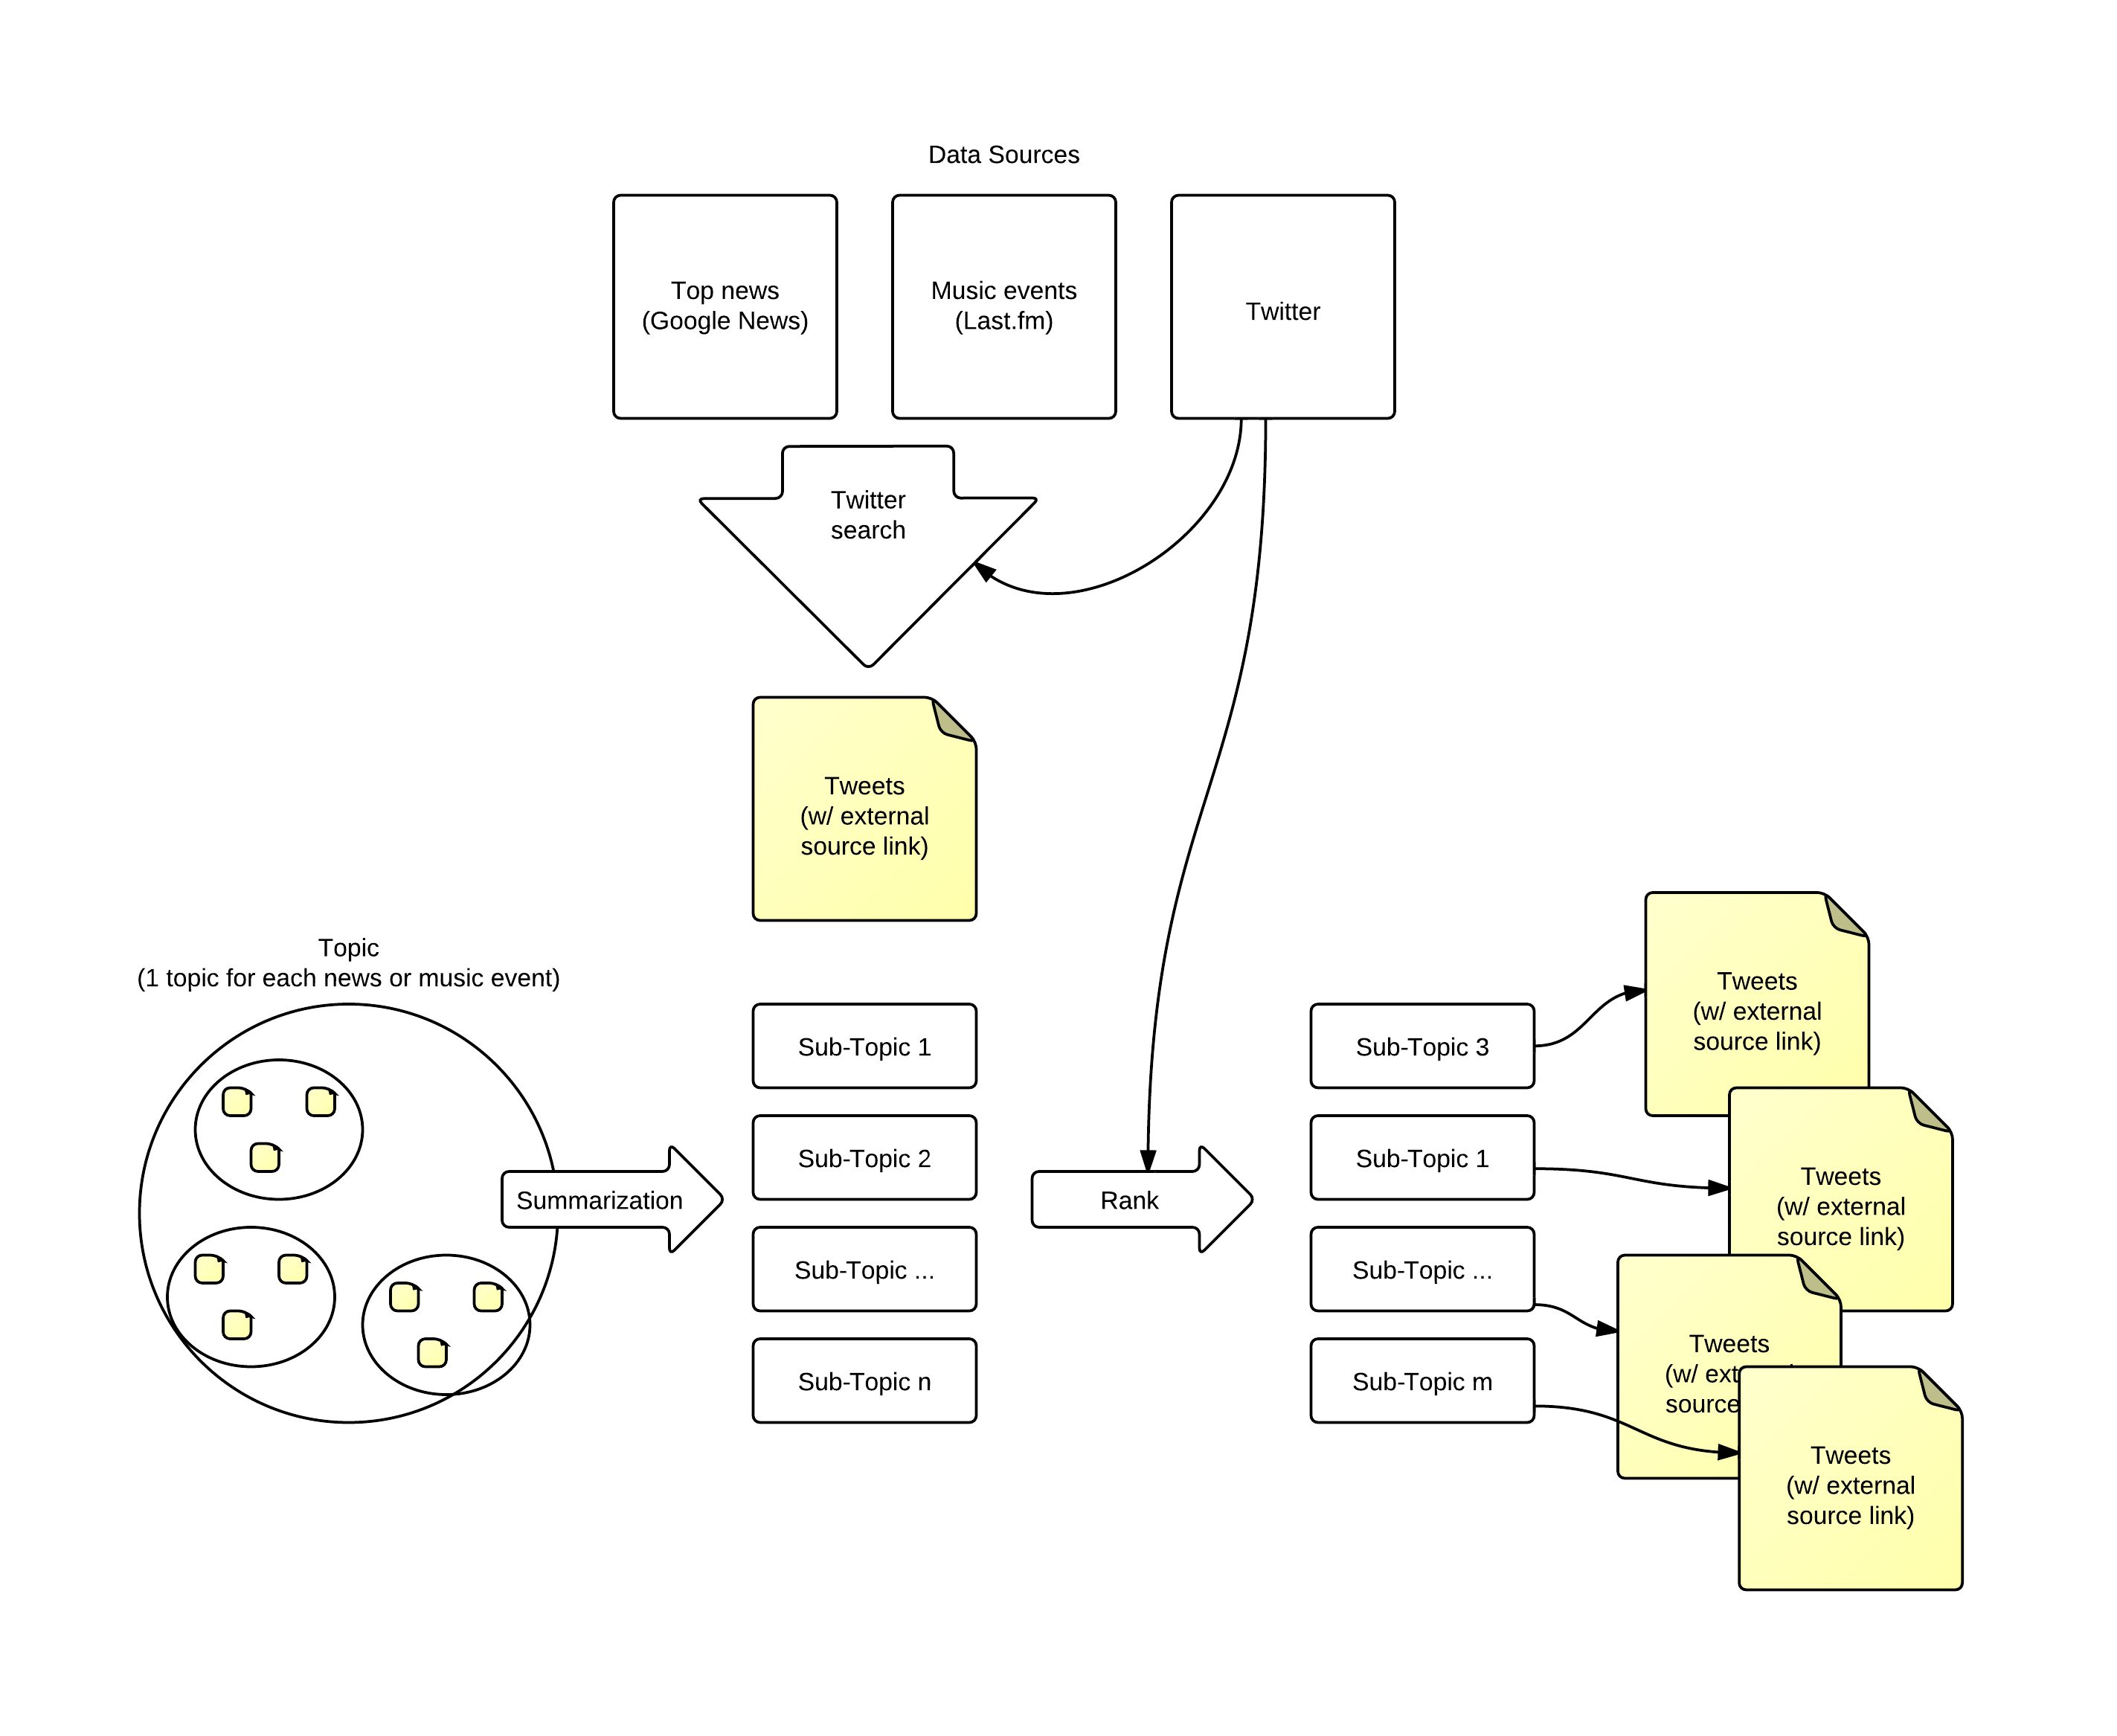
\includegraphics[width=15cm]{./img/general.png}
\caption{Diagrama descriptivo de la propuesta, sin la presentación de resultados.}
\end{figure}

   Como no se cuenta actualmente con un dataset de tamaño considerable para realizar el trabajo, se añade como una etapa inicial el obtener el conjunto de eventos. Luego, a partir de estos, se identifican los Objetos Web asociados, y luego se utilizarán enfoques similares a los empleados en \cite{events,clusterers} para resumir y hacer el ranking.\\

   La etapa siguiente de este proceso será identificar los \emph{Objetos Web} a partir del conjunto de documentos asociado a cada evento. Un Objeto Web $w$ se definirá como una entidad con ciertos atributos, tales como su Tipo (texto, imagen, audio o video), la URL que apunta al documento correspondiente $d$, y a un conjunto de \emph{Social Features} que será detallado más adelante. El objetivo de esta etapa es normalizar los datos obtenidos a partir del dataset inicial, debido al ruido usualmente encontrado en este tipo de datos.\\

   La parte esencial de los Objetos Web son sus Social Features, las cuales serán usadas para determinar su relevancia al momento de Resumir y Seleccionar contenido relevante de los eventos. Las Social Features son características asociadas a la URL del documento obtenidas a partir de fuentes sociales, tales como las redes sociales online. Entre estas características se cuentan:\\

\begin{enumerate}
\item cantidad de veces que se menciona la URL,
\item cantidad de personas distintas que mencionan la URL,
\item \emph{relevancia} de las personas que mencionan la URL,
\item \emph{relevancia} de la fuente de la URL,
\item cantidad de veces que se comparte la URL a partir de una misma mención,
\item rapidez con la que se viraliza la URL,
\item cobertura geográfica.
\end{enumerate}
   Algunas de estas características presentan desafíos en cómo definirlas y/o implementarlas, por ejemplo, la relevancia de las personas dependerá de muchos factores, todos dependientes de la plataforma de donde se obtengan estos datos, al igual que la relevancia de la fuente de cada URL y la disponibilidad de ciertos datos como la cobertura geográfica.\\

   La etapa de presentación de resultados consiste en implementar vistas para lo resultados obtenidos del proceso de resumen y ranking de los objetos más relevantes, de forma de apreciar empíricamente si los resultados coinciden con los eventos de los cuales fueron obtenidos.
  

\subsection{Desafíos previstos}
\label{sec-3.1}

\begin{enumerate}
\item Obtener una fuente de datos con los requisitos impuestos en la sección anterior. Es decir, un conjunto de eventos donde en cada uno además hay un conjunto de documentos asociados. Además debe haber una masa crítica para obtener buenos resultados.
\item En Twitter, cada URL mencionada es acortada usando un servicio propio de la plataforma, por lo que resolver la URL a la cual se referencia cada link acortado es una tarea costosa en tiempo y es un factor a considerar.
\item Detección de cuasi-duplicados: si bien dos URLs idénticas apuntan al mismo recurso, es posible que dos URLs distintas también lo hagan (por ejemplo, a la misma imagen). Un desafío será determinar una forma de identificar y agrupar este tipo de documentos.
\end{enumerate}
\subsection{Prueba de concepto}
\label{sec-3.2}


   Se obtuvo un dataset de 2.3 millones de tweets a partir de la red social Twitter, utilizando su Streaming API\footnote{\href{https://dev.twitter.com/docs/streaming-api}{https://dev.twitter.com/docs/streaming-api} }. De estos, aproximadamente 350 mil tweets incluían un enlace a otro sitio web en su mensaje. El siguiente desafío fue obtener las fuentes de esos enlaces, dado que la plataforma de Twitter utiliza un servicio de ``acortamiento'' de enlaces\footnote{\href{http://t.co/}{http://t.co/} }, por lo que el obtener la fuente de tales enlaces fue una tarea que tomó cierto tiempo comparado con el resto del análisis\footnote{Obtener los 2.3 millones de tweets tomó aproximadamente 22 horas, mientras que resolver las URLs acortadas tomó alrededor de 24 horas, a una tasa de 5 enlaces por segundo. }.\\

   En el siguiente histograma se aprecia la frecuencia de enlaces con respecto a los distintos dominios de la red.\\

   \begin{figure}[htb]
\centering
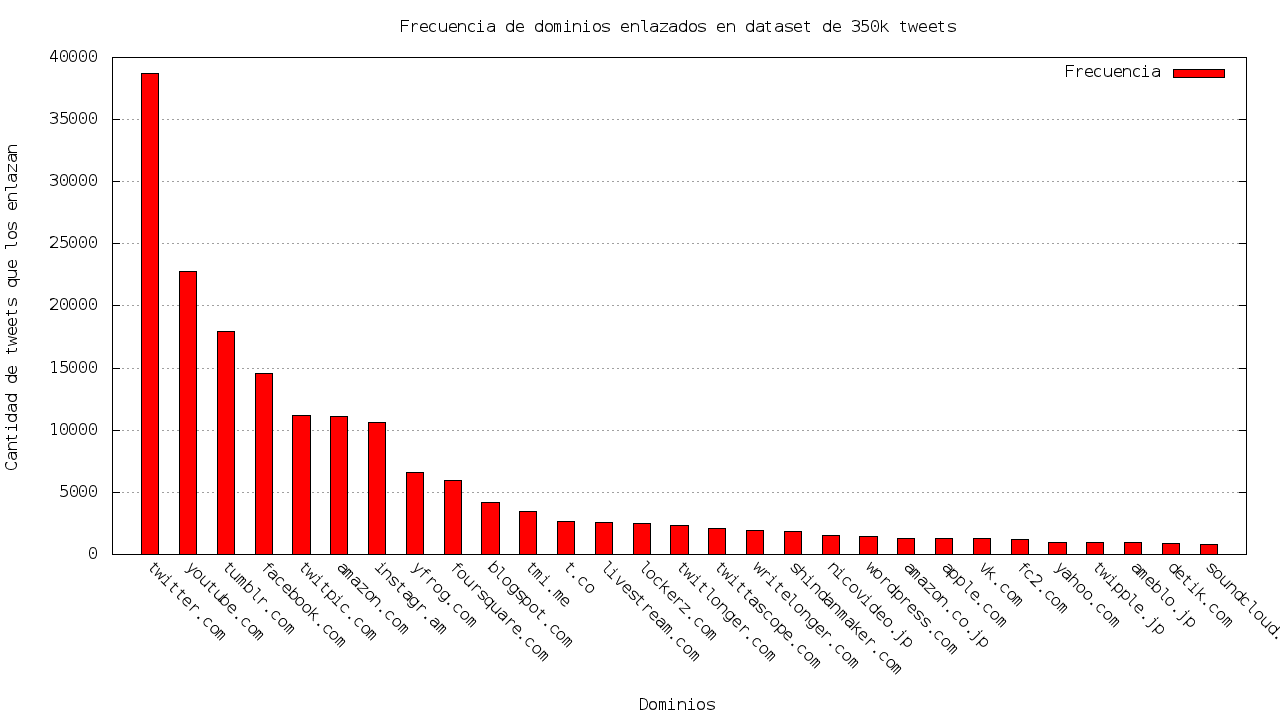
\includegraphics[width=15cm]{./img/dominios.png}
\caption{Histograma de frecuencia de dominios en dataset de tweets con enlaces}
\end{figure}
   
   La mayoría de los enlaces corresponden a la misma red social, lo que corresponde principalmente a enlaces a imágenes subidas al servicio y a actualizaciones de estado (enlaces que apuntan a otro tweet). A continuación siguen YouTube (videos), Facebook (imágenes, páginas, grupos, actualizaciones de estado, etc.), Tumblr (usualmente para publicar una nueva entrada en el blog, o para referenciar imágenes), Twitpic (imágenes), Amazon (enlaces a productos o imágenes), Instagram (imágenes), YFrog (imágenes), Foursquare (check-in en lugares físicos), Blogspot (publicar una nueva entrada, comentar un post o referenciar una imagen), etc. Una mención especial al servicio SoundCloud al final de la lista, cuya función es almacenar y compartir \emph{sonidos}.\\

   Dentro de la mayoría de los sitios asociados a los enlaces, se encuentran servicios de video, imágenes y de contenido multimedia (en el caso de los blogs como Tumblr, Blogspot o Wordpress).\\

   En la Figura 3 se aprecia la tasa de crecimiento de enlaces con respecto al tamaño del dataset obtenido hasta ese momento, mostrando un aumento lineal en la ocurrencia de enlaces a medida que crece el dataset. Según la documentación de la Streaming API, el método utilizado para obtener los tweets obtiene un \emph{muestreo} de los tweets publicados desde el momento de su invocación, mostrando, en caso de ser válida esa información, que el número de enlaces es proporcional al tamaño del dataset.\\

   \begin{figure}[htb]
\centering
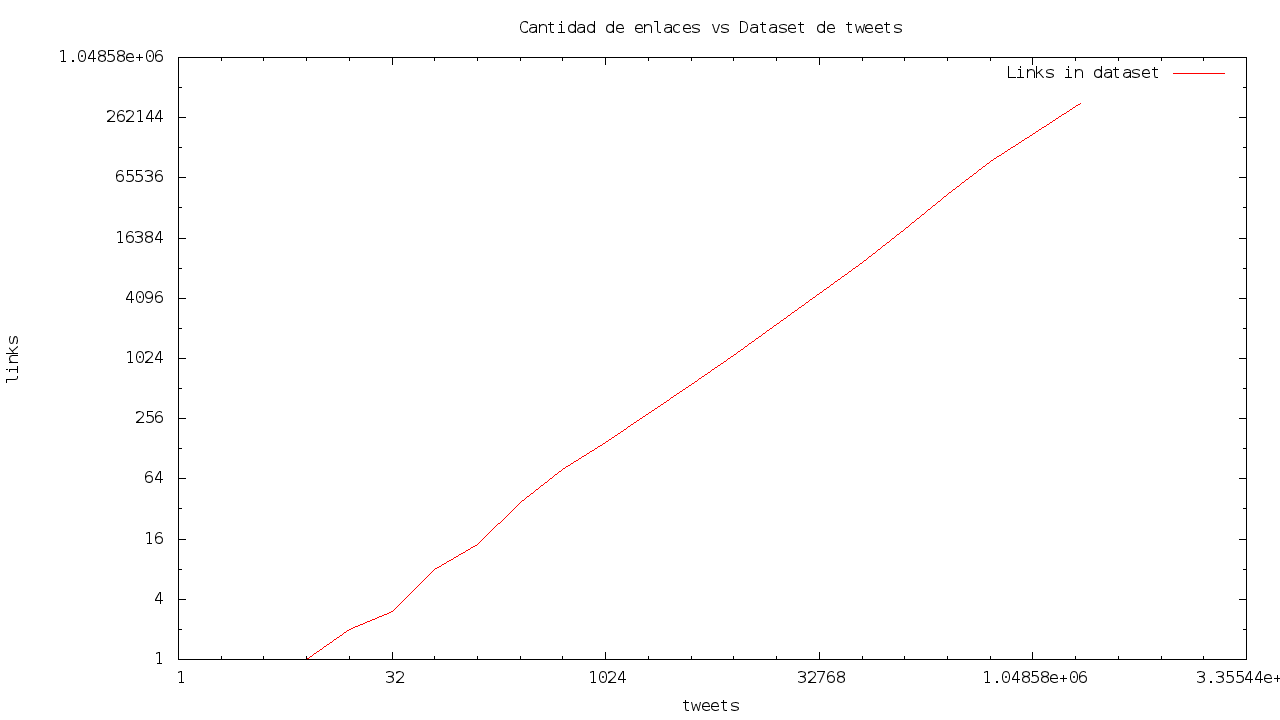
\includegraphics[width=15cm]{./img/links.png}
\caption{Gráfico log-log del crecimiento de la ocurrencia de enlaces con respecto al tamaño del dataset. Se aprecia un aumento lineal en la cantidad de enlaces con respecto al tamaño del dataset.}
\end{figure}

\newpage
\section{Objetivos}
\label{sec-4}

\subsection{Objetivo general}
\label{sec-4.1}

   A partir de un dataset de eventos definido en base a la red Twitter, el objetivo es determinar el contenido multimedia relevante de acuerdo a cada uno de estos eventos, implementando una estrategia de clustering y de resumen de eventos, presentando los resultados en un prototipo funcional.

\subsection{Objetivos específicos}
\label{sec-4.2}

\begin{itemize}
\item Comprobar la hipótesis de que es posible adaptar técnicas y herramientas para resumir y seleccionar contenido relevante para contenido multimedia, no solamente texto.
\item Determinar las características sociales más importantes en un objeto web para determinar su relevancia.
\item Diseñar e implementar una estrategia de Clustering para ordenar los objetos asociados a un evento y poder seleccionar los más relevantes, .
\item Diseñar e implementar un algoritmo de resumen (\emph{summarization}), basándose en \cite{events} para resumir el contenido de los eventos en contenido multimedia, adaptando los algoritmos para medir la similitud usando las características sociales de los objetos.
\item Diseñar una interfaz para presentar los resultados obtenidos luego del proceso de resumen y selección.
\end{itemize}
\newpage
\section{Plan de trabajo}
\label{sec-5}



\subsection{Obtención del Dataset inicial}
\label{sec-5.1}


    Se utilizará la API de Twitter para obtener tanto la información social como los recursos asociados a los eventos. Sin embargo, es necesario tener un conjunto de descripciones de eventos \emph{a priori} para poder obtener los recursos asociados. Se han considerado distintas alternativas hasta el momento:

\begin{enumerate}
\item Obtener información de eventos musicales utilizando la API de Last.fm\footnote{\href{http://www.lastfm.es/api/show/event.getInfo}{http://www.lastfm.es/api/show/event.getInfo} }, y luego generar automáticamente consultas a partir de esta información en Twitter, de una forma similar a como fue hecho en \cite{concerts}.
\item Utilizando un trabajo ya existente que consiste en un buscador de Tweets a partir de noticias en el servicio Google News\footnote{\href{http://news.google.com}{http://news.google.com} }, determinar un conjunto de noticias de alto impacto y obtener todos los tweets asociados a ellas.
\end{enumerate}
\subsection{Identificación de los Objetos Web y sus características sociales}
\label{sec-5.2}


    A partir de los eventos con sus respectivos recursos, identificar las características sociales relevantes a utilizar y calcularlas para cada recurso, lo cual puede ser costoso en tiempo dado que hay que visitar muchas URLs.

\subsection{Diseño e implementación de las estrategias de clustering y summarization}
\label{sec-5.3}


    Adaptar un algoritmo existente o diseñar e implementar una estrategia de Ranking y Resumen utilizando los features de cada objeto y su información social.

\subsection{Experimentación y ajustes de los algoritmos}
\label{sec-5.4}


    Determinar los mejores parámetros para los algoritmos y realizar experimentaciones, validando empíricamente su validez.

\subsection{Creación de una interfaz para visualizar y evaluar los resultados mediante un grupo de prueba}
\label{sec-5.5}


    Presentar los resultados obtenidos mediante una interfaz simple y usable, de forma de ver el contenido multimedia más importante a partir de un conjunto de eventos. Mediante un pequeño conjunto de usuarios, evaluar y validar los resultados obtenidos.



\newpage
\begin{thebibliography}{9}
\bibitem{concerts} 

Hila Becker, Dan Iter, Mor Naaman, Luis Gravano. \emph{Identifying Content for Planned Events Across Social Media Sites}. WSDM'12.

\bibitem{events}

Deepayan Chakrabarti, Kunal Punera. \emph{Event Summarization using Tweets}. AAAI 2011.

\bibitem{clusterers}

Hila Becker, Mor Naaman, Luis Gravano. \emph{Learning Similarity Metrics for Event Identification in Social Media}. WSDM'10.

\bibitem{selecting}

Hila Becker, Mor Naaman, Luis Gravano. \emph{Selecting Quality Twitter Content for Events}. AAAI 2011.

\bibitem{real}

Hila Becker, Mor Naaman, Luis Gravano. \emph{Beyond Trending Topics: Real-World Event Identification on Twitter}. AAAI 2011.

\end{thebibliography}









\end{document}
